\documentclass[conference]{IEEEtran}
\IEEEoverridecommandlockouts
% The preceding line is only needed to identify funding in the first footnote. If that is unneeded, please comment it out.
\usepackage{cite}

\usepackage{amsmath,amssymb,amsfonts}
\usepackage{algorithmic}
\usepackage{graphicx}
\usepackage{textcomp}
\usepackage{xcolor}
\usepackage{pifont}
\usepackage{float}

\newcommand{\xmark}{\ding{55}}%
\newcommand{\cmark}{\ding{51}}%

\def\BibTeX{{\rm B\kern-.05em{\sc i\kern-.025em b}\kern-.08em
    T\kern-.1667em\lower.7ex\hbox{E}\kern-.125emX}}
\begin{document}

\title{Analyzing Hardware Parameters for GPU based HPC Platform\\
%{\footnotesize \textsuperscript{*}Note: Sub-titles are not captured in Xplore and
%should not be used}
%\thanks{Identify applicable funding agency here. If none, delete this.}
}

\author{\IEEEauthorblockN{Saptarshi Bhowmik}
\IEEEauthorblockA{
\textit{Florida State University}\\
bhowmik@cs.fsu.edu}
\and
\IEEEauthorblockN{Nikhil Jain}
\IEEEauthorblockA{
\textit{NVIDIA Inc.}\\
nikhijain@nvidia.com}
\and
\IEEEauthorblockN{Abhinav Bhatele}
\IEEEauthorblockA{
\textit{University of Maryland}\\
bhatele@cs.umd.edu}
\and
\IEEEauthorblockN{Xin Yuan}
\IEEEauthorblockA{
\textit{Florida State University}\\
xyuan@cs.fsu.edu}
}

\maketitle

\begin{abstract}
In today's world, , for increasing the computational capacity of a compute node and reducing the number of endpoints in an interconnect network, more number of HPC Platforms are switching to GPU based compute nodes. However, the actual performance of HPC system all together, is affected by various other environment and hardware parameters. Here, in this poster we are studying the effect of one crucial hardware parameter 1) Link Bandwidth and one simulation environment of 2)GPUs per node, on the performance of few common HPC applications, in the context of two popular topology - Fat Tree\cite{b1} and 1D - Dragonfly\cite{b2}.  
\end{abstract}

\begin{IEEEkeywords}
performance, GPU per node, interconnect
\end{IEEEkeywords}

\section{Introduction}


Currently deployed networks are trying to reduce the number of endpoints by leveraging the GPU based compute nodes. These new GPU based compute nodes have larger computational prowess compared to a traditional CPU based compute nodes. However, there has been a continual discrepancy of computation and communication performance, with later, growing at a much slower rate. Along with that, increasing number of modern accelerations further dwindles this ratio. As such, there is a need to identify the environment and hardware specifications to make best possible use of the available system, and have a ideal communication/computation balance.  

\section{Methods}

\subsection{Trace Collection}

We use 6 representative applications for our experiments. We profile and collect the traces for these applications using Score-P\cite{b3}.

\subsection{TraceR-CODES}

We use the discrete event driven simulator, TraceR-CODES\cite{b4} to replay the application traces. The simulator network model is used to implement the interconnect topology, on top of which the traces are replayed.

\subsection{Network Topologies}

We use two popular interconnect topology 1D-Dragonfly and Fat-Tree for all our simulation\cite{b5}. For 1D-Dragonfly, we start our simulation with 16 groups and 1 GPU per compute node. We then reduce the size of the network to 8 group for 2 GPUs per compute node, 4 group for 4 GPUs per compute node and 1 group for 8 GPUs per compute node. For Fat-Tree, we start with 8 pods for 1 GPU per compute node  and keep on reducing the number of pods as we increase the number of GPUs per compute node. Ultimately have four configurations for Fat-Tree 8 pods for 1 GPU per compute node, 4 pods for 2 GPU per compute node, 2 pods for 4 GPU per compute node and 1 pods for 8 GPU per compute node.

\subsection{Bandwidth}

We set the base bandwidth(x) for the Links as 11.9 Gb/s, which is the link bandwidths used in Quartz machines, and keep the internal bandwidth as 23.8 GB/sec. We use 8 more bandwidth, x/16, x/8, x/4, x/2, 2x, 4x, 8x, 16x,  which are a proportion of the base bandwidths, for our simulations.

\subsection{GPUs per node}
 
We are using 1 GPU per node for a maximum sized network and then we are subsequently increasing it to 2 GPUs per node, 4 GPUs per node and 8 GPUs per node, with reducing the network size simultaneously.

\subsection{Workload}

We are running 20 Workloads of randomly selected jobs from the six application listed in the table below, from ranks 32, 64, 128, 256 and 512. We make sure that each rank of an application appears at least 4 times throughout all the 20 workloads.

\begin{table}[htbp]
\caption{Application Traces}
%\begin{adjustbox}{width=\columnwidth,left}
\begin{center}
\begin{tabular}{|c|c|c|} \hline

\hline
\textbf{Traces} & \textbf{Computation} & \textbf{Communication} \\ \hline
Stencil4d & \xmark & \cmark  \\    \hline
Kripke & \cmark & \xmark  \\    \hline
Laghos & \cmark & \xmark  \\    \hline
Subcomm-a2a & \xmark & \cmark  \\    \hline
Sw4lite & \cmark  & \cmark  \\    \hline
Amg & \cmark  & \cmark  \\    \hline
\end{tabular}
\label{tab1}
\end{center}
\end{table}

\section{Result}
\subsection{Impact of GPUs per Node}\label{AA}
The below results show application speedup with respect to the default setting is 1 GPU per Node. 
\begin{figure}[H]
\centering
\centering
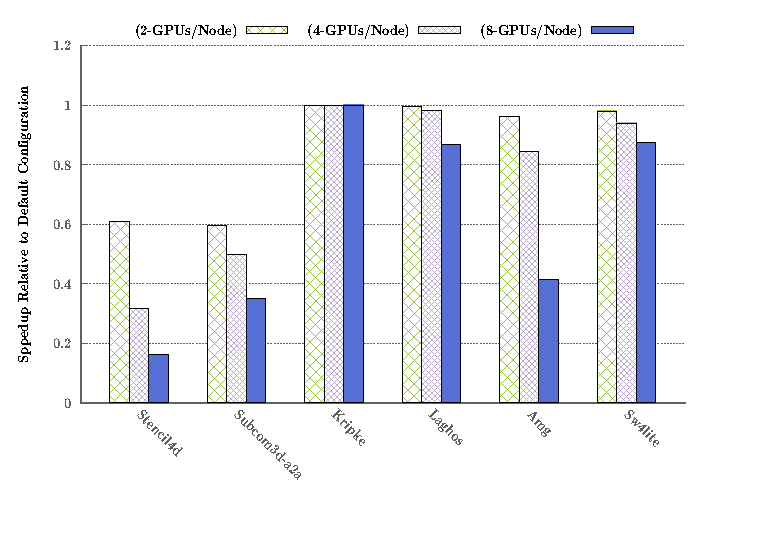
\includegraphics[width=1\linewidth, height=5cm]{figs/dfly-x-mapping-all.eps}
%\captionsetup{labelformat=empty}
\caption{Different GPUs per node mapping for all Applications of 128 ranks in 1D-Dragonfly}
\end{figure}

\begin{figure}[H]
\centering
\centering
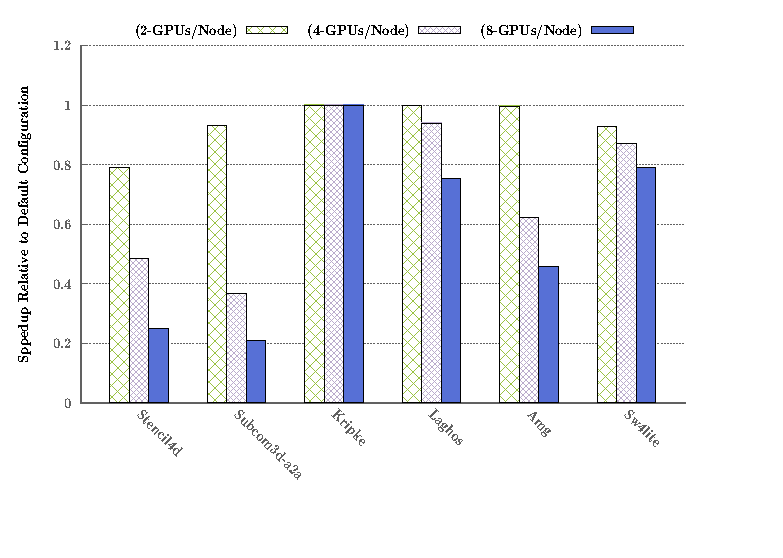
\includegraphics[width=1\linewidth, height=5cm]{figs/ftree-x-mapping-all.eps}
%\captionsetup{labelformat=empty}
\caption{Different GPUs per node mapping for all Applications of 128 ranks in Fat-Tree}
\end{figure}

Communication intensive applications experience more slowdown than applications with computation.

\subsection{Impact of Bandwidth}
The below results show application speedup with respect to the default setting is 1 GPU per Node and Link Bandwidth 11.9 Gb/s
\begin{figure}[H]
\centering
\centering
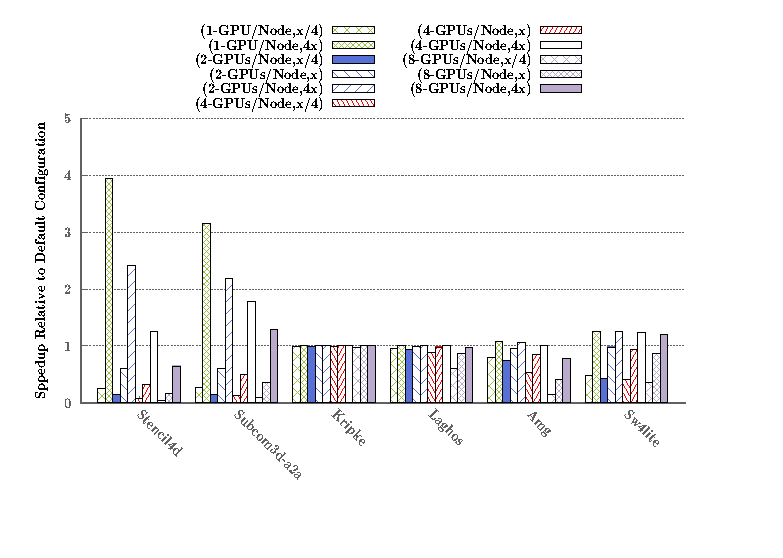
\includegraphics[width=1\linewidth, height=5cm]{figs/dfly-bw-mapping-all.eps}
%\captionsetup{labelformat=empty}
\caption{Different Bandwidth and GPUs per node mapping for all Applications of 128 ranks in 1D-Dragonfly}
\end{figure}

\begin{figure}[H]
\centering

\centering
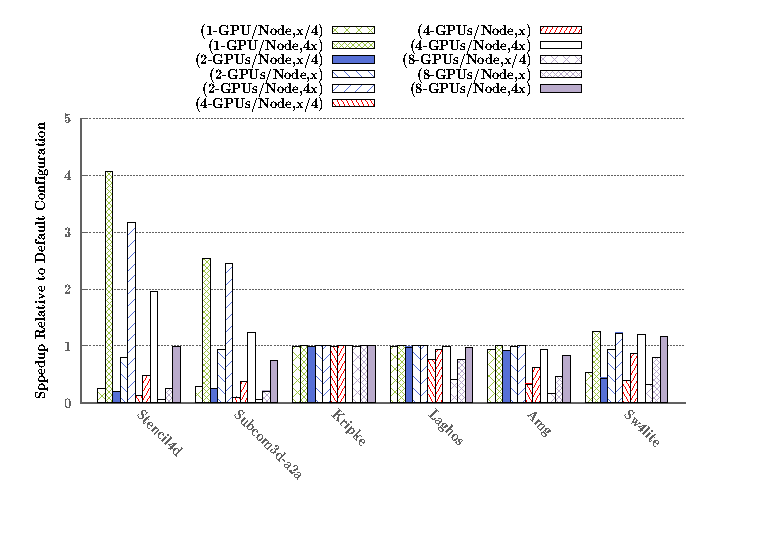
\includegraphics[width=1\linewidth, height=5cm]{figs/ftree-bw-mapping-all.eps}
%\captionsetup{labelformat=empty}
\caption{Different  Bandwidth and GPUs per node mapping for all Applications of 128 ranks in Fat-Tree}

\end{figure}

Applications performance speedup when the bandwidth is increased.
The increase is more pronounced is full computational intensive applications.

\section{Conclusion}
\begin{itemize}
    \item As the number of GPU per node increases, the node becomes more intensive, and thus, there is a slowdown in application performance as the communication/computation capacity of the network reduces.
    \item As the number of GPU per node increases, more bandwidth is needed to substantiate the slowdown in application performance.
    \item Every application has a sweet spot where it is performing the best.
\end{itemize}

\section{Future Works}
\begin{itemize}
    \item Study how other simulation environment and hardware design, such as NIC scheduling policies effect the performance of applications

    \item Profile more HPC applications and find the performance of those applications across the currently deployed GPU based interconnect topology,
\end{itemize}


\begin{thebibliography}{00}
\bibitem{b1} Jain, N., Bhatele, A., Howell, L. H., Böhme, D., Karlin, I., León, E. A., ... & Leininger, M. L. (2017, November). Predicting the performance impact of different fat-tree configurations. In Proceedings of the International Conference for High Performance Computing, Networking, Storage and Analysis (pp. 1-13).
\bibitem{b2} Kim, J., Dally, W. J., Scott, S., & Abts, D. (2008, June). Technology-driven, highly-scalable dragonfly topology. In 2008 International Symposium on Computer Architecture (pp. 77-88). IEEE.
\bibitem{b3} Knüpfer, A., Rössel, C., an Mey, D., Biersdorff, S., Diethelm, K., Eschweiler, D., ... & Nagel, W. E. (2012). Score-p: A joint performance measurement run-time infrastructure for periscope, scalasca, tau, and vampir. In Tools for High Performance Computing 2011 (pp. 79-91). Springer, Berlin, Heidelberg.
\bibitem{b4} Acun, B., Jain, N., Bhatele, A., Mubarak, M., Carothers, C. D., & Kale, L. V. (2015, August). Preliminary evaluation of a parallel trace replay tool for hpc network simulations. In European Conference on Parallel Processing (pp. 417-429). Springer, Cham.
\bibitem{b5} Alzaid, Z. S. A., Bhowmik, S., Yuan, X., & Lang, M. (2020, June). Global link arrangement for practical Dragonfly. In Proceedings of the 34th ACM International Conference on Supercomputing (pp. 1-11). Magnetics Japan, p. 301, 1982].

\end{thebibliography}
\vspace{12pt}
\end{document}
